% Template for Cogsci submission with R Markdown

% Stuff changed from original Markdown PLOS Template
\documentclass[10pt, letterpaper]{article}

\usepackage{cogsci}
\usepackage{pslatex}
\usepackage{float}
\usepackage{caption}

% amsmath package, useful for mathematical formulas
\usepackage{amsmath}

% amssymb package, useful for mathematical symbols
\usepackage{amssymb}

% hyperref package, useful for hyperlinks
\usepackage{hyperref}

% graphicx package, useful for including eps and pdf graphics
% include graphics with the command \includegraphics
\usepackage{graphicx}

% Sweave(-like)
\usepackage{fancyvrb}
\DefineVerbatimEnvironment{Sinput}{Verbatim}{fontshape=sl}
\DefineVerbatimEnvironment{Soutput}{Verbatim}{}
\DefineVerbatimEnvironment{Scode}{Verbatim}{fontshape=sl}
\newenvironment{Schunk}{}{}
\DefineVerbatimEnvironment{Code}{Verbatim}{}
\DefineVerbatimEnvironment{CodeInput}{Verbatim}{fontshape=sl}
\DefineVerbatimEnvironment{CodeOutput}{Verbatim}{}
\newenvironment{CodeChunk}{}{}

% cite package, to clean up citations in the main text. Do not remove.
\usepackage{cite}

\usepackage{color}

% Use doublespacing - comment out for single spacing
%\usepackage{setspace}
%\doublespacing


% % Text layout
% \topmargin 0.0cm
% \oddsidemargin 0.5cm
% \evensidemargin 0.5cm
% \textwidth 16cm
% \textheight 21cm

\title{An information-seeking account of eye movements during spoken and signed
language comprehension}


\author{ {\large \bf Kyle MacDonald}$^1$ (kylem4@stanford.edu), {\large \bf Aviva Blonder}$^2$ (aviva.blonder@oberlin.edu), \\  {\large \bf Virginia Marchman}$^1$ (marchman@stanford.edu), {\large \bf Anne Fernald}$^1$ (afernald@stanford.edu), \\ {\large \bf Michael C. Frank}$^1$ (mcfrank@stanford.edu)  \\
   $^1$ Department of Psychology Stanford University, $^2$ Department of Psychology Oberlin College}

\begin{document}

\maketitle

\begin{abstract}
Language comprehension in grounded contexts involves integrating visual
and linguistic information through decisions about visual fixation. But
when the visual signal also contains information about the language
source -- as in the case of facial expressions, written text, or sign
language -- then any choice of a fixation target can involve a tradeoff
between gathering information about language or exploring the
nonlinguistic visual context. In the current work, we explore this
tradeoff and hypothesize that human eye-movement patterns represent an
adaptive response. We use two case studies of eye movements during
language comprehension to test predictions of our account. First, we
show that, compared to children processing spoken language, young sign
language learners (a) delayed eye movements away from a language source,
(b) were more accurate with their initial shifts, and (c) produced a
smaller proportion of nonlanguage-driven gaze shifts (E1). Next, we
present a well-controlled, confirmatory test of our adaptive tradeoff
account, showing that English-speaking adults produced fewer
nonlanguage-driven eye movements when processing displays of printed
text compared to spoken language (E2). Together, these data suggest that
people adapt to the value of seeking different information in order to
increase the chance of rapid and accurate language understanding.

\textbf{Keywords:}
eye movements; language processing; information-seeking; American Sign
Language
\end{abstract}

\section{Introduction}\label{introduction}

Language comprehension involves quickly integrating the linguistic
signal with information about the surrounding visual world. But in some
contexts, the visual world can also provide information that is directly
related to the linguistic signal. For example, imagine that a speaker
asks you to ``Pass the salt'' but there is noise in the surrounding
context, making it difficult to understand the request. Here,
comprehension can be facilitated by (a) fixating on the nonlinguistic
visual world (i.e., encoding the objects that are present in the scene)
or (b) fixating on source of the language: the speaker (i.e., reading
lips or perhaps the direction of gaze). However, this situation creates
a tradeoff where the listener must decide what kind of information to
gather and at what time. How do we decide when to fixate on the language
source and when to gather information about the nonlinguistic visual
world?

We propose that people modulate their eye movement behavior in response
to changes in the value of gathering different kinds of information. We
test this information-seeking account using two case studies that
manipulate the value of different fixation locations in the visual world
for language understanding: a) a comparison of processing a
visual-manual vs.~a spoken language in children (Experiment 1), and b) a
comparison of processing printed text vs.~spoken language in adults
(Experiment 2).

The study of eye movements during language comprehension has provided
insight into the interaction between conceptual representations of the
world and the incoming linguistic signal. For example, research shows
that adults and children will rapidly shift visual attention upon
hearing the name of an object in the visual scene, with a high
proportion of these shifts occurring prior to the offset of the target
word (Allopenna, Magnuson, \& Tanenhaus, 1998; Tanenhaus,
Spivey-Knowlton, Eberhard, \& Sedivy, 1995). Moreover, researchers have
found that conceptual representations activated by fixations to the
visual world can modulate subsequent eye movements during language
processing (Altmann \& Kamide, 2007). The majority of this work has
leveraged eye movements as the output of the underlying language
comprehension process, using linguistic stimuli that comes from a
disembodied voice. But this work has focused less on contexts where the
visual world also provides an opportunity to gather information about
the linguistic signal by fixating on the language source.

In contrast, researchers in the fields of natural vision have modeled
fixations to the visual world as a tool for information gathering
(Hayhoe \& Ballard, 2005). In this approach, eye movements reflect a
goal to gather information to reduce uncertainty and to maximize the
expected reward of future actions. For example, Hayhoe \& Ballard (2005)
review evidence that people do not fixate on the most salient aspects of
a visual scene, but instead focus on aspects that are most helpful for
the current task such as choosing to fixate on an upcoming obstacle when
walking.

In the current work, we leverage aspects of this information-seeking
framework to account for a wider variety of fixation patterns during
language comprehension. We characterize eye movements as a tradeoff
between gathering information about the nonlinguistic visual world and
monitoring the incoming linguistic signal. We assume that the goal is to
maximize the chance of making a correct future response (in the context
of our task, resolving reference rapidly and accurately by looking at
the object that is being talked about). To test the predictions of our
account, we present two case studies where information about the
linguistic signal can be gathered via fixations to the language source:
processing American Sign Language (ASL) and processing displays of
printed text. Our key prediction is that competition for visual
attention will make eye movements away from the language source less
valuable than fixating the source of the linguistic signal, leading
people to generate fewer exploratory, nonlanguage-driven shifts.

\begin{CodeChunk}
\begin{figure}[t]

{\centering 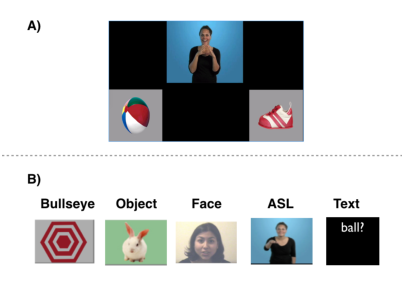
\includegraphics{figs/e1_stimuli-1} 

}

\caption[Stimuli for Experiments 1 and 2]{Stimuli for Experiments 1 and 2. Panel A shows the layout of the three potential fixation locations across all the tasks: the center stimulus, the target picture, and the distracter picture. Panel B shows the five different center stimulus items from Experiments 1 and 2: a person signing (ASL), a person speaking (Face), a static image of a familiar object (Object), a static geometric shape (Bullseye), and printed text (Text).}\label{fig:e1_stimuli}
\end{figure}
\end{CodeChunk}

\section{Experiment 1}\label{experiment-1}

E1 provides an initial test of our information-seeking account. We
directly compared eye movements of children learning ASL to children
learning a spoken language using parallel, 3-alternative forced choice
real-time language comprehension tasks. The spoken language data are a
reanalysis of three unpublished data sets, and the ASL data are reported
in MacDonald et al. (under review). We predicted that, compared to
spoken language processing, processing ASL would increase the value of
fixating on the language source and decrease the value of generating
exploratory, nonlanguage-driven shifts.

To test this prediction, we present standard behavioral analyses of
Accuracy and RT. We also present two exploratory model-based analyses:
An exponentially weighted moving average (EWMA) method (Vandekerckhove
\& Tuerlinckx, 2007) that categorizes gaze shifts as either
language-driven or random guessing. Then, for the shifts flagged as
language-driven by the EWMA model, we fit drift-diffusion models (DDMs)
(Ratcliff \& Childers, 2015) to quantify differences in the dynamics of
speed and accuracy of eye movements.

Since our results are complex, we preview them here: when the center
stimulus was an Object or a Bullseye, kids' first shifts away from the
center stimulus were fast and at chance, and models suggested they never
stopped guessing even when the language was informative. In contrast,
for the Face condition and even more so for the signers, kids fixated on
the speaker to gather information and generated more accurate first
shifts. In other words, their eye movements reflected a tradeoff between
the value of gathering information from the speaker and exploring the
nonlinguistic visual world.

\subsection{Method}\label{method}

\subsubsection{Participants}\label{participants}

\begin{table}[b]
\centering
\begin{tabular}{lrrrr}
  \hline
Task & Mean\_Age & Min\_Age & Max\_Age & n \\ 
  \hline
ASL & 27.60 &  16 &  53 &  27 \\ 
  Face & 26.00 &  25 &  26 &  24 \\ 
  Object & 31.90 &  26 &  39 &  40 \\ 
  Bullseye & 26.10 &  26 &  27 &  16 \\ 
   \hline
\end{tabular}
\caption{Age distributions of children in Experiment 1.} 
\end{table}

Table 1 contains details about the age distributions of children in all
of four samples.

\emph{Spoken English samples.} Participants were 80 native, monolingual
English-learning children divided across three samples. Participants had
no reported history of developmental or language delay.

\emph{ASL sample.} Participants were 27 native, monolingual ASL-learning
children (14 deaf, 13 hearing). All children, regardless of hearing
status, were exposed to ASL from birth through extensive interaction
with at least one caregiver fluent in ASL and were reported to
experience at least 80\% ASL in their daily lives. The ASL sample
included a wider age range compared to the spoken English samples
because this population is difficult to recruit.

\subsubsection{Stimuli}\label{stimuli}

\emph{ASL linguistic stimuli.} We recorded two sets of ASL stimuli,
using two valid ASL sentence structures for questions: 1)
Sentence-initial wh-phrase: ``HEY! WHERE {[}target noun{]}?'' and 2)
Sentence-final wh-phrase: ``HEY! {[}target noun{]} WHERE?'' Two female
native ASL users recorded several tokens of each sentence in a
child-directed register. Before each sentence, the signer produced a
hand-wave gesture commonly used in ASL to gain an interlocutor's
attention before initiating an utterance.

\emph{English linguistic stimuli.} All three tasks (Object, Bullseye,
and Face) featured the same female native speaker of English. The
speaker used natural child-directed speech and said: ``Look! Where's the
(target word)?'' The target words were: ball, banana, book, cookie,
juice, and shoe. For the Face task, a female native English speaker was
video-recorded as she looked straight ahead and said, ``Look! Where's
the (target word)?''

\emph{ASL and English visual stimuli.} The image set consisted of
colorful digitized pictures of objects presented in fixed pairs with no
phonological overlap (ASL task: cat---bird, car---book, bear---doll,
ball---shoe; English tasks: book-shoe, juice-banana, cookie-ball).
Images were digitized pictures presented in fixed pairs matched for
visual salience. Side of target picture was counterbalanced across
trials.

\subsubsection{Design and procedure}\label{design-and-procedure}

Children sat on their caregiver's lap and viewed the task on a screen
while their gaze was recorded using a digital camcorder. On each trial,
pictures of two familiar objects appeared and between the two pictures
was a central stimulus (ASL, Face, Object, or Bullseye). Participants
saw approximately 32 test trials with several filler trials interspersed
to maintain children's interest.

\emph{Trial structure.} On each trial, children saw two images of
familiar objects on the screen for two seconds before the center
stimulus appeared. Then they processed the target sentence -- which
consisted of a carrier phrase, a target noun, and a question -- followed
by two seconds without language to allow for a response.

\emph{Coding.} Participants' gaze patterns were coded (33-ms resolution)
as being fixated on either the center stimulus, one of the images,
shifting between pictures, or away.

\subsubsection{Behavioral measures}\label{behavioral-measures}

\emph{Reaction time.} Reaction time (RT) corresponds to the latency to
shift from the central stimulus to either the target or the distracter
pictures measured from target-noun onset. We chose to exclude RTs longer
than two seconds since these shifts are unlikely to be generated in
response to the incoming language stimulus (see Ratcliff, 1993).

\emph{First shift accuracy.} Accuracy was the mean proportion of first
shifts that landed on the target picture out of the total number of
shifts that landed on either the target or the distracter picture over a
two-second window from target noun onset.

\begin{CodeChunk}
\begin{figure}[t]

{\centering 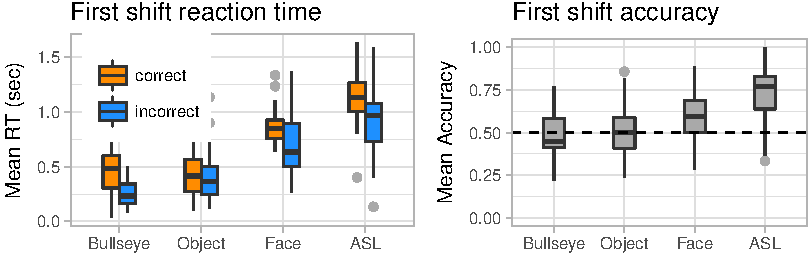
\includegraphics{figs/e1_acc_rt_plot-1} 

}

\caption[First shift accuracy and Reaction times (RT) from E1]{First shift accuracy and Reaction times (RT) from E1. Panel A shows a boxplot representing the distribution of RTs for correct (orange) and incorrect (blue) shifts for each center stimulus type. Panel B shows the distribution of mean first shift accuracy scores for each center stimulus type. The solid lines represent median values, the boundaries of the box show the upper and lower quartiles, and the whiskers show the full range of the data excluding outliers.}\label{fig:e1_acc_rt_plot}
\end{figure}
\end{CodeChunk}

\begin{CodeChunk}
\begin{figure}[t]

{\centering 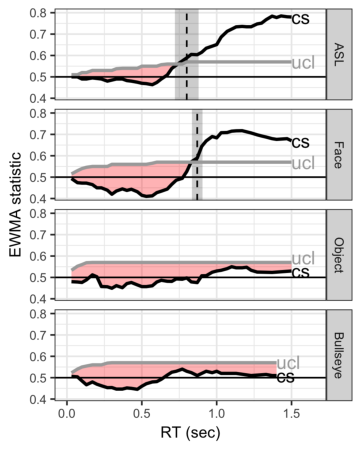
\includegraphics{figs/e1_control_chart-1} 

}

\caption[Output for the EWMA guessing model for all center stimulus types in E1]{Output for the EWMA guessing model for all center stimulus types in E1. The black curve represents the evolution of the control statistic (CS) as a function of reaction time. The grey curve represents the upper control limit (UCL). The vertical dashed line is the median cutoff value (point when the control process shifts out of a guessing state) across all participants. The grey shaded area represents the 95\% confidence interval around the estimate of the median cutoff point. And the shaded red area represents the proprotion of responses that were flagged as guesses by the EWMA model.}\label{fig:e1_control_chart}
\end{figure}
\end{CodeChunk}

\begin{CodeChunk}
\begin{figure}[t]

{\centering 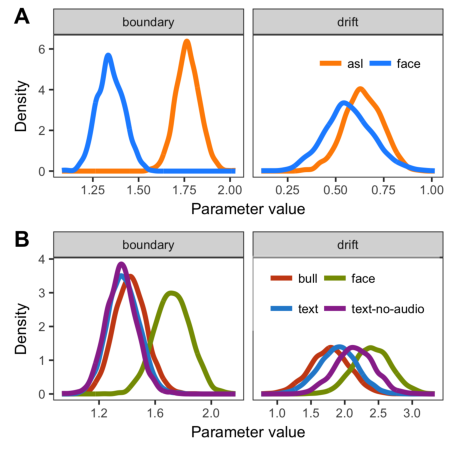
\includegraphics{figs/hddm_plot-1} 

}

\caption[Posterior distributions over the boundary and drift rate parameters in the heirarchical drift diffusion model for Experiment 1 (Panel A) and 2 (Panel B)]{Posterior distributions over the boundary and drift rate parameters in the heirarchical drift diffusion model for Experiment 1 (Panel A) and 2 (Panel B).}\label{fig:hddm_plot}
\end{figure}
\end{CodeChunk}

\subsection{Results and Discussion}\label{results-and-discussion}

\subsubsection{Analysis plan}\label{analysis-plan}

First, we present behavioral analyses of Accuracy and RT. We log
transformed all RTs and used the \texttt{lme4} R package (Bates,
Maechler, Bolker, \& Walker, 2013) to fit mixed-effects regression
models that included a by-subject random intercept for each participant.
All data and analysis code can be found in the online repository for
this project: \url{https://github.com/kemacdonald/speed-acc}.

Next, we present two exploratory model-based analyses to quantify
differences in eye movements across the four samples. First, we use an
EWMA method to model changes in accuracy as a function of increases in
RT. For each RT, the model generates two values: a ``control statistic''
(CS, which captures the running average of first shift accuracy) and an
``upper control limit'' (UCL, which captures the pre-defined limit of
when accuracy is categorized as above chance level). Here, the CS is an
expectation of random shifting to either the target or the distracter
image, or a Bernoulli process with probability of success 0.5. As the
RTs get longer, we assume that participants have gathered more
information and should become more accurate, or a Bernoulli process with
probability success \textgreater{} 0.5. Using this model, we can
quantify and compare: a) the cutoff point when the CS exceeds the UCL,
indicating that participants started to generate language-driven shifts
and b) the proportion of shifts that the model categorizes as
language-driven vs.~nonlanguage-driven.

Finally, we took the language-driven shifts from the EWMA and fit a
hierarchical Bayesian drift-diffusion model (HDDM) to quantify
differences in the speed and accuracy of language-driven eye movements.
We chose to implement a hierarchical Bayesian version of the DDM using
the HDDM Python package (Wiecki, Sofer, \& Frank, 2013) since we had
relatively few trials from child participants and recent simulation
studies have shown that the HDDM approach was better than other DDM
fitting methods for small data sets (Ratcliff \& Childers, 2015).{]}.
The model assumes that people accumulate noisy evidence in favor of one
alternative with a response generated when the evidence crosses a
pre-defined decision threshold. Here we focus on two parameters of
interest that map onto meaningful psychological variables:
\textbf{boundary separation}, which indexes the amount of evidence
gathered before generating a response (higher values suggest a
prioritization of accuracy over speed) and \textbf{drift rate}, which
indexes the amount of evidence that is accumulated per unit time (higher
values suggest more efficient processing).

\subsubsection{Behavioral analyses}\label{behavioral-analyses}

\emph{RT.} Visual inspection of the Figure 2 panel A suggests that there
was a speed accuracy tradeoff in the ASL, Face, and Bullseye conditions,
with incorrect RTs tended to be faster than correct RTs. To quantify
differences across the groups, we fit a linear mixed-effects regression
predicting first shift RT as a function of center stimulus type,
controlling for age, and including user-defined contrasts to test
specific comparisons of interest:
\texttt{Log(RT) $\sim$ center stimulus type + age +  (1 | subject)}. We
found that (a) ASL learners generated slower RTs compared to all of the
spoken English samples (\(\beta\) = -0.96, \(p\) \textless{} .001), (b)
ASL learners' shifts were slower compared directly to participants in
the Face task (\(\beta\) = -0.42, \(p\) \textless{} .001), and (c)
participants in the Face task shifted slower compared to participants in
the Object and Bullseye tasks (\(\beta\) = -0.73, \(p\) \textless{}
.001).

\emph{Accuracy.} Next we compared the accuracy of first shifts across
the different tasks by fitting a mixed-effects logistic regression with
the same specifications and contrasts as the RT model. We found that (a)
ASL learners were more accurate compared to all of the spoken English
samples (\(\beta\) = -0.69, \(p\) \textless{} .001), (b) ASL learners
were more accurate when directly compared to participants in the Face
task (\(\beta\) = -0.54, \(p\) = 0.001), and (c) participants in the
Face task were numerically more accurate compared to participants in the
Object and Bullseye tasks (\(\beta\) = -0.73) but this effect was not
significant (\(p\) = 0.094).

\subsubsection{Model-based analyses}\label{model-based-analyses}

\emph{EWMA.} Figure 3 shows changes in the control statistic (CS) and
the upper control limit (UCL) as a function of participants' RTs. Each
CS starts at chance performance and below the UCL. In the ASL and Face
tasks, the CS value begins to increase with RTs around 0.7 seconds after
noun onset and eventually crosses the UCL, indicating that responses
\textgreater{} 0.7 sec were on average above chance levels. In contrast,
the CS in the Object and Bullseye tasks never crossed the UCL,
indicating that children's shifts were equally likely to land on the
target or the distracter, regardless of when they were initiated. This
result suggests that first shifts in the Bullseye/Object tasks were not
language-driven and may instead reflect a different process such as
gathering more information about the referents in the visual world.

Next, we compared the EWMA output for participants in the ASL and Face
tasks. We found that ASL learners generated fewer shifts when the CS was
below the UCL (\(\beta\) = -1.64, \(p\) \textless{} .001), indicating
that a larger proportion of their initial shifts away were
language-driven (see the differences in the red shaded area in Figure
3). We did not find evidence for a difference in the timing of when the
CS crossed the UCL (\(\beta\) = -0.03, \(p\) = 0.576), indicating that
both groups began to generate language-driven shifts about the same time
after noun onset.

\emph{HDDM.} Using the output of the EWMA, we compared the timing and
accuracy of language-driven shifts for participants in the ASL and Face
tasks.\footnote{We did interpret the DDM fits for the Bullseye/Face
  tasks since there was suggestion of any non-guessing signal.} We found
that ASL learners had a higher estimate for the boundary separation
parameter compared to the Face participants (ASL boundary = 1.77, HDI =
{[}1.64, 1.9{]}; Face boundary = 1.35, HDI = {[}1.21, 1.49{]}), with no
overlap in the credible values (see Figure 4). This suggests that ASL
learners accumulated more evidence about the linguistic signal before
generating an eye movement. We found high overlap for estimates of the
drift rate parameter, indicating that both groups processed the
linguistic information with similar efficiency (ASL drift = 0.64, HDI =
{[}0.44, 0.83{]}; Face drift = 0.57, HDI = {[}0.33, 0.83{]}).

Taken together, the behavioral analyses and the EWMA/HDDM results
provide converging support that ASL learners were sensitive to the value
of eye movements, producing fewer nonlanguage-driven shifts and
prioritizing accuracy over speed, but accumulating information at
roughly the same rate. This behavior seems reasonable since the
potential for missing subsequent linguistic information is high if ASL
users shifted prior to gathering sufficient information. It is important
to point out that these were exploratory findings and that there were
several, potentially important differences between the stimuli,
apparatus, and populations. Thus, we set out to perform a
well-controlled, confirmatory test of our account in E2.

\section{Experiment 2}\label{experiment-2}

\begin{CodeChunk}
\begin{figure}[t]

{\centering 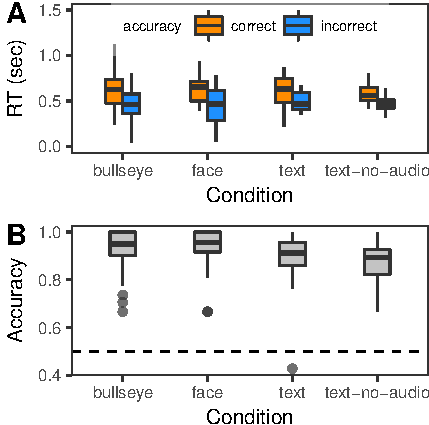
\includegraphics{figs/e2_plot_print-1} 

}

\caption[Behavioral results from E2 for all center stimulus types]{Behavioral results from E2 for all center stimulus types. Panel A shows reaction times, and Panel B shows accuracy. All plotting conventions are the same as in Figure 2.}\label{fig:e2_plot_print}
\end{figure}
\end{CodeChunk}

\begin{CodeChunk}
\begin{figure}[t]

{\centering 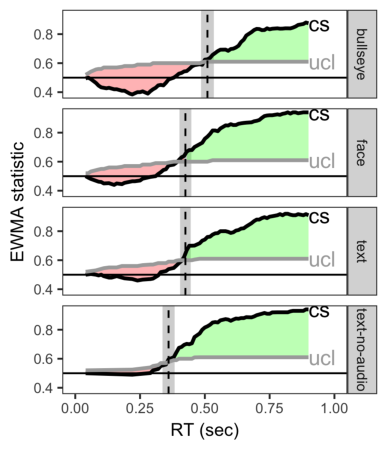
\includegraphics{figs/e2_control_chart-1} 

}

\caption[EWMA model output from E2]{EWMA model output from E2. All plotting conventions are the same as Figure 3.}\label{fig:e2_control_chart}
\end{figure}
\end{CodeChunk}

In E2, we attempt to replicate a key finding from E1: that increasing
the competition between fixating the language source and the
nonlinguistic visual world reduces nonlanguage-driven eye movements.
Moreover, we set out to conduct a confirmatory test of our hypothesis
that also controlled for the population differences present in E1. We
tested a sample of English-speaking adults using a within-participants
manipulation of the center stimulus type. We used the Face and Bullseye
stimulus sets from E1 and added two new conditions: Text, where the
verbal language information was accompanied by a word-by-word display of
printed text (see Figure 1)), and Text-no-audio, where the spoken
language stimulus was removed. We chose text processing since, like sign
language comprehension, the linguistic information is gathered via
fixations to the visual world.

Our key behavioral prediction is that participants in the Text
conditions should produce a higher proportion of language-driven shifts
as indexed by the EWMA model output. We also predicted to find no
differences in the DDM parameter fits since the manipulation modulates
participants' strategic allocation of visual attention and not the
accuracy/efficiency of information processing.

\subsection{Method}\label{method-1}

\subsubsection{Participants}\label{participants-1}

25 Stanford undergraduates participated (6 male, 20 females) for course
credit. All participants were monolingual, native English speakers and
had normal vision.

\subsubsection{Stimuli}\label{stimuli-1}

Audio and visual stimuli were identical to the Face and Bullseye tasks
in E1. We included a new center fixation stimulus type: printed text.
The text was displayed in a white font on a black background and was
programmed such that only a single word appeared on the screen, with
each word appearing for the same duration as the corresponding word in
the spoken language stimuli.

\subsubsection{Design and procedure}\label{design-and-procedure-1}

The design was nearly identical to E1, with the exception of a change to
a within-subjects manipulation where each participant completed all four
tasks (Bullseye, Face, Text, and Text-no-audio). In the Text condition,
spoken language accompanied the printed text. In the Text-no-audio
condition, the spoken language stimulus was removed. Participants saw a
total of 128 trials while their eye movements were tracked using
automated eye-tracking software.

\subsection{Results and Discussion}\label{results-and-discussion-1}

\subsubsection{Behavioral analyses}\label{behavioral-analyses-1}

\emph{RT.} Visual inspection of Figure 5 panel A suggests that there was
a speed-accuracy tradeoff for all conditions: incorrect RTs tended to be
faster than correct RTs. We fit a linear mixed-effects regression with
the same specification as in E1, but we added by-subject intercepts and
slopes for each center stimulus type to account for our within-subjects
manipulation. We did not find evidence that RTs were different across
conditions (all \(p\) \textgreater{} .05).

\emph{Accuracy.} Next, we modeled accuracy using a mixed-effects
logistic regression with the same specifications (see Panel B of Figure
5). We found that participants tended to be less accurate in the Text
conditions compared to conditions without text (\(\beta\) = -0.62, \(p\)
\textless{} .001). We did not any other statisically significant
differences.

\subsubsection{Model-based analyses}\label{model-based-analyses-1}

\emph{EWMA.} For all four conditions, the CS crossed the UCL (see panel
C of Figure 5), suggesting that adults' shifts were language-driven.
Interestingly, we found a graded effect of condition on the RT when the
CS crossed the UCL such that the Text-no-audio condition occurred
earliest (see the vertical dashed lines in Figure 5), followed by the
Text and Face conditions that were not different from one another, and
finally the Bullseye condition (TODO stats). We also found the same
graded difference in the proportion of shifts that occurred while the CS
was below the UCL, indicating a higher proportion of first shifts were
language-driven in the Text conditions, with the highest proportion in
the Text-no-audio condition (TODO stats). These results provide strong
evidence for our key prediction: that increasing the value of fixating
the language source reduces gaze shifts to the nonlinguistic visual
world.

\emph{HDDM.} Using the output of the EWMA, we fit the same hierarchical
DDM as in E1 to test if there were differences in the timing and
accuracy of responses generated by the incoming linguistic signal. There
was a high overlap of the posterior distributions for boundary
separation and drift rate (STATS TODO), suggesting that participants
gathered similar amounts of information before generating a response and
processed the information with similar efficiency.

Together, these results suggest that participants were sensitive to the
tradeoff between gathering visual information about the language source
versus the nonlinguistic visual world. When processing text, adults
generated fewer nonlanguage-driven shifts (EWMA results) but did not
change the amount of information gathered or the efficiency of
processing the linguistic signal itself (HDDM results). Interestingly,
we even found a graded difference between the Text and Text-no-audio
conditions, with the lowest proportion of nonlanguage-driven shifts
occurring in the Text-no-audio condition. This behavior makes sense if
hearing adults could rely on the auditory channel to gather the
linguistic information, then they do not have to allocate as many visual
fixations to the text display.

\section{General Discussion}\label{general-discussion}

During real world language comprehension, eye movements to the source of
language can provide additional information about the linguistic signal.
But this creates a tradeoff between fixating on a source of linguistic
information and fixating on the nonlinguistic visual world. In the
current work, we propose that eye movements during language processing
reflect a sensitivity to the value of gathering different kinds of
information. We found that young ASL-learners generated slower but more
accurate shifts away from a language source and produced a smaller
proportion of nonlanguage-driven shifts. We found the same pattern of
behavior within a sample of English-speaking adults processing displays
of printed text compared to spoken language. These results suggest that
as the value of fixating on a location to gather information about
language increases, eye movements to gather information about the visual
world become less useful and occur less often.

Our work here attempts to synthesize results from different populations
and stimuli in a single framework, but it has several limitations that
we hope will pave the way for future work. First, we have not performed
a confirmatory test of the DDM findings (ASL-learners prioritize
accuracy over speed) from E1. So this finding, while interesting, is
preliminary. Second, we do not know what might be driving the population
differences in E1. It could be that ASL-learners massive experience
dealing with competition for visual attention leads to changes in the
deployment of eye movements during language comprehension. Or, it could
be that the in-the-moment constraints of processing a visual language
cause different fixation behavior. Finally, we used a very simple visual
world, with only three places to look, and very simple linguistic
stimuli, especially for the adults in E2. Thus it remains an open
question how these results might scale up to more complex language
information and visual environments.

A strength of this work is the attempt to integrate top-down, goal-based
models of vision with work on language-driven eye movements. While we
chose to start with two particular case studies -- ASL and text
processing -- we think the account is more general and that there are
many real world situations where people must negotiate the tradeoff
between gathering more information about language or about the world:
e.g., processing spoken language in noisy environments or at a distance;
or early in language learning when children are acquiring new words and
often rely on nonlinguistic cues to reference such as pointing or eye
gaze. Overall, we hope this work contributes to a broader account of eye
movements during language comprehension that can explain fixation
behaviors across a wider variety of populations, processing contexts,
and during different stages of language learning.

\section{Acknowledgements}\label{acknowledgements}

We are grateful to the families who participated in this research and to
the California School for the Deaf in Fremont for their help with
participant recruitment. This work was supported by a National Science
Foundation Graduate Research Fellowship to KM and an NIDCD grant to Anne
Fernald and David Corina (DC012505).

\section{References}\label{references}

\setlength{\parindent}{-0.1in} \setlength{\leftskip}{0.125in} \noindent

\hypertarget{refs}{}
\hypertarget{ref-allopenna1998tracking}{}
Allopenna, P. D., Magnuson, J. S., \& Tanenhaus, M. K. (1998). Tracking
the time course of spoken word recognition using eye movements: Evidence
for continuous mapping models. \emph{Journal of Memory and Language},
\emph{38}(4), 419--439.

\hypertarget{ref-altmann2007real}{}
Altmann, G., \& Kamide, Y. (2007). The real-time mediation of visual
attention by language and world knowledge: Linking anticipatory (and
other) eye movements to linguistic processing. \emph{Journal of Memory
and Language}, \emph{57}(4), 502--518.

\hypertarget{ref-bates2013lme4}{}
Bates, D., Maechler, M., Bolker, B., \& Walker, S. (2013). Lme4: Linear
mixed-effects models using eigen and s4. r package version 1.0-5.

\hypertarget{ref-hayhoe2005eye}{}
Hayhoe, M., \& Ballard, D. (2005). Eye movements in natural behavior.
\emph{Trends in Cognitive Sciences}, \emph{9}(4), 188--194.

\hypertarget{ref-macdonald2017realtime}{}
MacDonald, K., LaMarr, T., Corina, D. and, Marchman, V., \& Fernald, A.
(under review). Real-time lexical comprehension in young children
learning american sign language.

\hypertarget{ref-ratcliff2015individual}{}
Ratcliff, R., \& Childers, R. (2015). Individual differences and fitting
methods for the two-choice diffusion model of decision making.
\emph{Decision}, \emph{2}(4), 237--279.

\hypertarget{ref-salverda2011goal}{}
Salverda, A. P., Brown, M., \& Tanenhaus, M. K. (2011). A goal-based
perspective on eye movements in visual world studies. \emph{Acta
Psychologica}, \emph{137}(2), 172--180.

\hypertarget{ref-tanenhaus1995integration}{}
Tanenhaus, M. K., Spivey-Knowlton, M. J., Eberhard, K. M., \& Sedivy, J.
C. (1995). Integration of visual and linguistic information in spoken
language comprehension. \emph{Science}, \emph{268}(5217), 1632.

\hypertarget{ref-vandekerckhove2007fitting}{}
Vandekerckhove, J., \& Tuerlinckx, F. (2007). Fitting the ratcliff
diffusion model to experimental data. \emph{Psychonomic Bulletin \&
Review}, \emph{14}(6), 1011--1026.

\hypertarget{ref-wiecki2013hddm}{}
Wiecki, T. V., Sofer, I., \& Frank, M. J. (2013). HDDM: Hierarchical
bayesian estimation of the drift-diffusion model in python.
\emph{Frontiers in Neuroinformatics}, \emph{7}, 14.

\end{document}
